\documentclass[11pt,a4paper]{article}

\usepackage[utf8]{inputenc}
\usepackage[T1]{fontenc}
\usepackage[spanish,es-nodecimaldot]{babel}
\usepackage{lmodern}
\usepackage{microtype}
\usepackage[a4paper,margin=2.35cm]{geometry}
\usepackage{graphicx}
\usepackage{booktabs}
\usepackage{tabularx}
\usepackage{array}
\usepackage{float}
\usepackage{xcolor}
\usepackage{fancyhdr}
\usepackage{enumitem}
\usepackage[hidelinks]{hyperref}

\graphicspath{{images/}}
\definecolor{spotifygreen}{HTML}{198A45}
\definecolor{spotifydark}{HTML}{1E2823}
\definecolor{softgray}{HTML}{F2F5F3}
\newcommand{\code}[1]{\texttt{\detokenize{#1}}}
\renewcommand{\arraystretch}{1.14}
\setlength{\parindent}{0pt}
\setlength{\parskip}{0.52em}
\setlength{\emergencystretch}{3em}
\setlist{nosep,leftmargin=*}
\pagestyle{fancy}
\fancyhf{}
\lhead{EA2 Spotify - informe de Lucas}
\rhead{Trabajo individual y traspaso}
\cfoot{\thepage}
\setlength{\headheight}{14pt}

\title{\textbf{Popularidad histórica de canciones}\\[0.3em]
\large Informe individual de modelamiento, evaluación y traspaso al equipo}
\author{Lucas Moncada\\Evaluación Parcial 2 - Machine Learning}
\date{24 de octubre de 2026}

\begin{document}
\maketitle

\begin{center}
\fcolorbox{spotifygreen}{softgray}{\parbox{0.89\linewidth}{
Este informe consolida el trabajo de Lucas y entrega a Ignacio y César las decisiones,
cifras, figuras y límites que deben poder reproducir y explicar. La evidencia ejecutable
es \path{notebooks/04a_modeling_lucas.ipynb}; el informe no sustituye al notebook
integrador ni al README Markdown exigido para la entrega del equipo.}}
\end{center}

\begin{abstract}
Se estudió si atributos musicales y géneros permiten estimar la popularidad histórica
de 89.740 canciones únicas de Spotify Tracks. Ridge completo obtuvo MAE 11,915,
RMSE 16,643 y $R^2=0,348$ en la prueba aleatoria, frente a MAE 17,250 de la
referencia mediana. Quitar los géneros elevó el MAE de Ridge a 16,671. Una prueba
separada por artista principal mantuvo MAE 12,102, con artistas secundarios
compartidos en parte de la prueba. El ranking del 10\,\% recuperó 159 de 653
canciones populares y omitió 494. K-Means produjo dos perfiles musicales amplios
cuya separación es modesta (silueta 0,245). Los hallazgos sirven para formular
auditorías de catálogo; no establecen causalidad ni anticipan el éxito futuro.
\end{abstract}

\tableofcontents
\clearpage
\section{Propósito y mapa de evidencias}

La pregunta supervisada es cuánto aportan el audio y los géneros a la estimación de
\code{popularity}, un valor histórico entre 0 y 100. La pregunta no supervisada es si
los atributos musicales permiten describir perfiles útiles para explorar el catálogo.
El KPI retrospectivo simula una capacidad de revisión del 10\,\% de la prueba y cuenta
cuántas canciones con \code{popularity >= 70} aparecen en esa lista. El valor real ya
existe en la fuente: el ejercicio no representa una decisión comercial lista para usar.

\begin{table}[htbp]
\centering\small
\begin{tabularx}{\linewidth}{>{\raggedright\arraybackslash}p{0.29\linewidth}X}
\toprule
Artefacto & Uso para Ignacio, César y el notebook integrador \\
\midrule
\path{docs/ea2/protocolo_comun.md} & Definiciones compartidas de datos, particiones, modelos y métricas. \\
\path{notebooks/04a_modeling_lucas.ipynb} & Cálculo reproducible, salidas, figuras e interpretación del trabajo de Lucas. \\
\path{src/spotify_popularity/modeling/protocol.py} & Funciones de partición, codificación, pipelines y métricas. \\
\path{docs/ea2/lucas.md} & Alcance individual y reproducción desde instalación limpia. \\
Este informe & Síntesis para revisión cruzada; las cifras oficiales del equipo se recalculan en el notebook 05. \\
\bottomrule
\end{tabularx}
\caption{Función de cada artefacto en el traspaso.}
\label{tab:mapa}
\end{table}

\section{Metodología, fuente y preparación}

El trabajo sigue CRISP-DM de manera verificable: pregunta y KPI para la
\emph{comprensión del negocio}; controles de la fuente y hallazgos de EP1 para la
\emph{comprensión de datos}; deduplicación y codificación para la \emph{preparación};
Ridge, árbol y K-Means para \emph{modelamiento}; pruebas, segmentos, ranking y
sensibilidades para \emph{evaluación}; notebook e informe para la entrega académica,
sin despliegue operativo. La evaluación retroalimenta la definición de uso: los
errores extremos impiden recomendar decisiones automáticas.

La fuente inmutable es \path{data/raw/Spotify_Tracks_Dataset.csv}, con SHA-256:

{\footnotesize\ttfamily\noindent b202fa49909b2d5cef71a04b1d21243cfeb36414535f2ca9272aa646721177bd\par}
De 114.000 filas se retiró una inválida y se consolidaron 24.259 repeticiones de
\code{track_id}; el procesado tiene 89.740 canciones únicas, 20 columnas y cero
faltantes. La popularidad queda en 0--100. EP1 encontró 10,47\,\% de ceros,
3,48\,\% de canciones con popularidad al menos 70 y asociaciones acústicas
individuales débiles. La fuente aportaba exactamente 1.000 filas por género antes
de consolidar duplicados; sus frecuencias no representan el catálogo natural.

\begin{figure}[htbp]
\centering
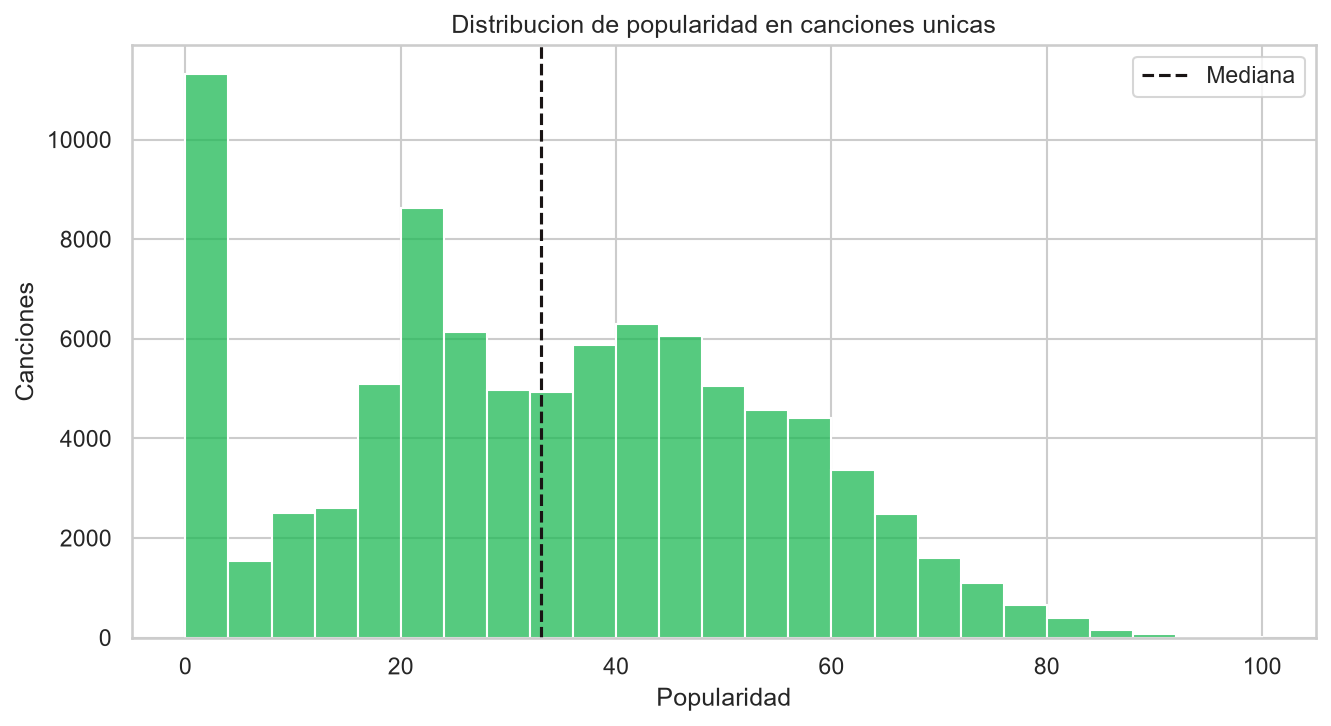
\includegraphics[width=0.81\linewidth]{05_processed_popularity_distribution.png}
\caption{Distribución de popularidad del procesado, proveniente del EDA de EP1. Los extremos justifican la referencia mediana y el diagnóstico por rangos.}
\label{fig:target}
\end{figure}

\begin{figure}[htbp]
\centering
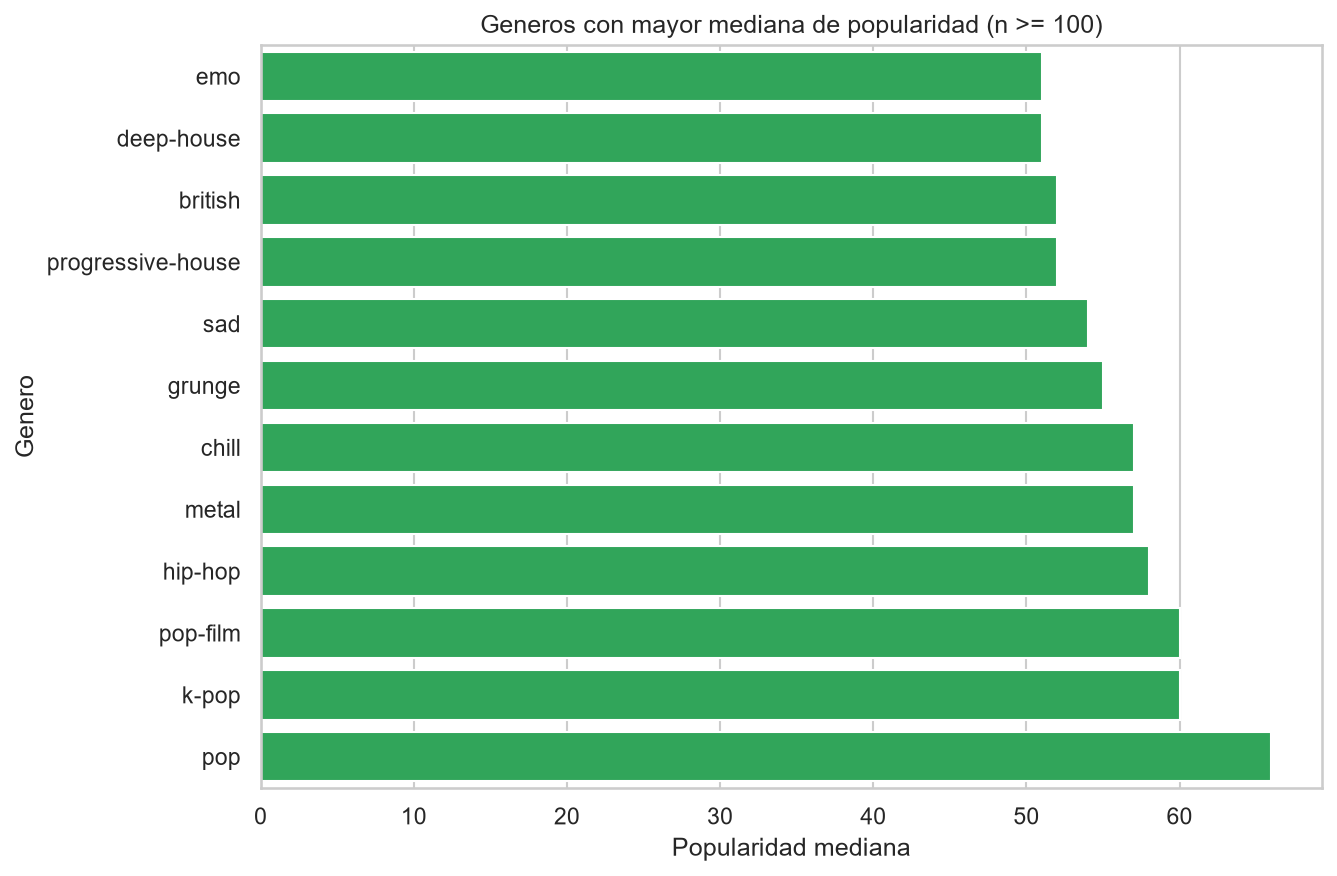
\includegraphics[width=0.81\linewidth]{09_genre_popularity_summary.png}
\caption{Resumen descriptivo por género elaborado en EP1. Su lectura está condicionada por el diseño de muestreo.}
\label{fig:genre-eda}
\end{figure}

\subsection{Partición común y prevención de fuga}

Se ordenaron los \code{track_id} únicos y se aplicó \code{train_test_split} con
\code{test_size=0.20}, semilla 42 y mezcla aleatoria. Quedaron 71.792 canciones
de entrenamiento y 17.948 de prueba. Del entrenamiento se apartó un 20\,\%
adicional: 57.433 para ajustar candidatos y 14.359 para validarlos. La huella
SHA-256 de los IDs ordenados de la prueba aleatoria es:

{\footnotesize\ttfamily\noindent 7270ff57b6fb81215fba2f834942d194183e3854ccac935a65e5a03f7888b318\par}
Los tres integrantes deben usar esos mismos IDs para la comparación principal.

El objetivo, \code{track_id}, nombres, álbum y artistas no entraron como predictores.
Las diez columnas numéricas fueron \code{duration_ms}, \code{danceability},
\code{energy}, \code{loudness}, \code{speechiness}, \code{acousticness},
\code{instrumentalness}, \code{liveness}, \code{valence} y \code{tempo}. Las
cuatro categóricas fueron \code{key}, \code{mode}, \code{time_signature} y
\code{explicit}. \code{track_genres} se separó por \code{|} y se codificó como
multietiqueta. Escalado, one-hot y codificación de géneros se ajustaron dentro de
cada pipeline usando solo la partición de entrenamiento correspondiente; las
etiquetas no vistas se ignoran.

\section{Aprendizaje supervisado}

\code{popularity} es numérica, por lo que se compararon regresores. Una referencia
\code{DummyRegressor} con estrategia mediana fija el MAE que deben superar. Ridge
ofrece una combinación lineal regularizada ante atributos correlacionados; el árbol
de regresión captura umbrales e interacciones, con riesgo de sobreajuste. Se probaron
\code{alpha} 0,1; 1; 10 y 100 para Ridge, y profundidades 5, 10 o 15 con hojas
mínimas de 20 o 100 para el árbol. La regla fue menor MAE de validación, luego RMSE
y menor complejidad. No se usó la prueba para elegir parámetros.

\begin{table}[htbp]
\centering\small
\begin{tabular}{llrrrl}
\toprule
Predictores & Modelo & MAE & RMSE & $R^2$ & Configuración \\
\midrule
Completo & Ridge & 11,786 & 16,430 & 0,360 & $\alpha=0,1$ \\
Completo & Árbol & 14,393 & 18,312 & 0,205 & prof. 15; hoja 20 \\
Sin géneros & Ridge & 16,581 & 20,162 & 0,036 & $\alpha=0,1$ \\
Sin géneros & Árbol & 15,627 & 19,830 & 0,067 & prof. 15; hoja 20 \\
\bottomrule
\end{tabular}
\caption{Configuraciones seleccionadas en validación aleatoria; la referencia tuvo MAE 17,208.}
\label{tab:validation}
\end{table}

Tras reajustar cada configuración con las 71.792 canciones de entrenamiento, Ridge
completo obtuvo el menor MAE de la prueba aleatoria, como muestra la
Tabla~\ref{tab:random-test}. MAE y RMSE se expresan en puntos de popularidad.
$R^2$ compara el error cuadrático con una predicción constante igual a la media
observada de la prueba.

\begin{table}[htbp]
\centering\small
\begin{tabular}{llrrrr}
\toprule
Predictores & Modelo & MAE & RMSE & $R^2$ & Mejora MAE \\
\midrule
Referencia & Mediana & 17,250 & 20,612 & $\approx 0$ & 0,000 \\
Completo & Ridge & 11,915 & 16,643 & 0,348 & 5,335 \\
Completo & Árbol & 14,508 & 18,460 & 0,198 & 2,742 \\
Sin géneros & Ridge & 16,671 & 20,223 & 0,037 & 0,580 \\
Sin géneros & Árbol & 15,693 & 19,834 & 0,074 & 1,557 \\
\bottomrule
\end{tabular}
\caption{Prueba aleatoria reservada, $n=17.948$. La mejora MAE se calcula frente a la referencia mediana de esta misma prueba.}
\label{tab:random-test}
\end{table}

\begin{figure}[htbp]
\centering
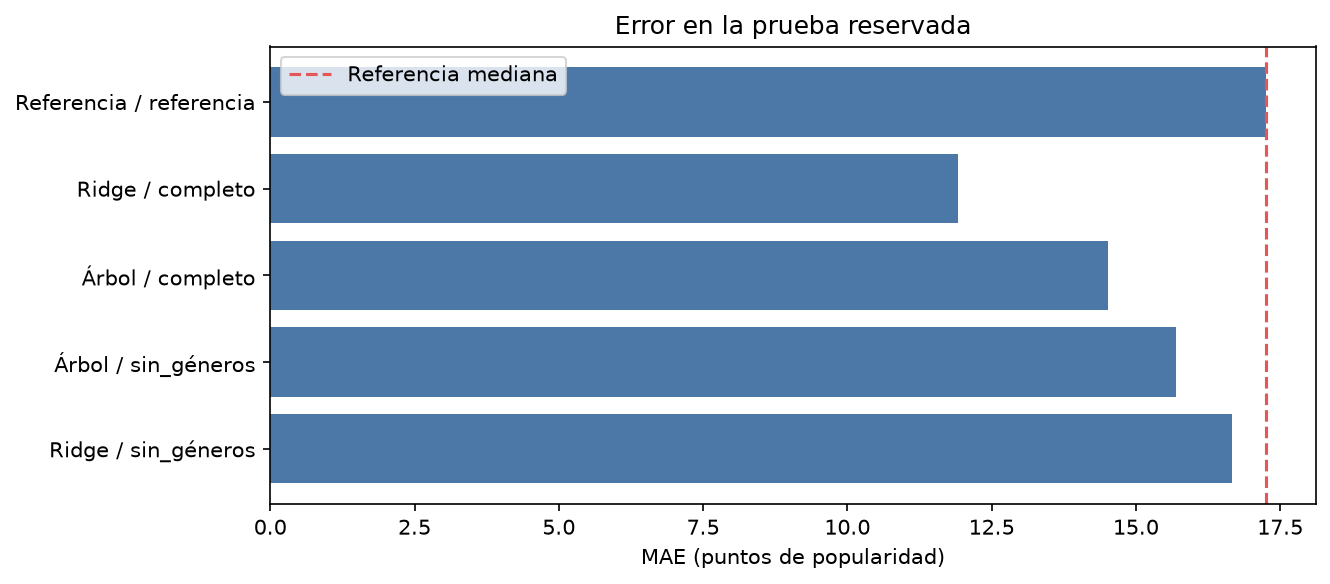
\includegraphics[width=0.91\linewidth]{04a_lucas_model_mae.png}
\caption{MAE de las configuraciones preseleccionadas en la prueba aleatoria. La línea vertical corresponde a la referencia mediana.}
\label{fig:model-mae}
\end{figure}

\subsection{Aporte de los géneros}

La ablación principal retira solo \code{track_genres} y conserva audio, estructura
musical y \code{explicit}. Bajo esa única diferencia, el MAE de Ridge aumenta
4,756 puntos (11,915 a 16,671) y el del árbol aumenta 1,186 (14,508 a 15,693).
En una comparación adicional \emph{solo de validación} se aislaron exactamente las
diez variables numéricas de audio, las etiquetas de género y ambas juntas; las
cuatro categóricas quedaron fuera para que los nombres de los conjuntos fueran
literales. Los mismos IDs y la misma regla de selección se usaron en cada variante.

\begin{table}[htbp]
\centering\small
\begin{tabular}{lrrrr}
\toprule
Variables & MAE Ridge & $R^2$ Ridge & MAE árbol & $R^2$ árbol \\
\midrule
Solo audio & 16,630 & 0,032 & 15,686 & 0,092 \\
Solo géneros & 11,849 & 0,355 & 14,472 & 0,204 \\
Audio y géneros & 11,800 & 0,358 & 14,391 & 0,204 \\
\bottomrule
\end{tabular}
\caption{Análisis adicional en los mismos 14.359 IDs de validación; no reabre la prueba aleatoria.}
\label{tab:feature-sets}
\end{table}

Con Ridge, añadir audio a solo géneros reduce el MAE de validación apenas 0,049
puntos. La señal de género sostiene casi todo el rendimiento de esa combinación
en esta muestra. No se puede cuantificar qué parte persistiría con una distribución
natural de géneros ni atribuir causalidad al género.

\section{Transferencia a artistas principales no vistos}

Como diagnóstico secundario se definió el grupo por el primer nombre de
\code{artists} antes de \code{;}, sin espacios laterales y sin distinguir
mayúsculas. \code{GroupShuffleSplit} con semilla 42 reservó 18.193 canciones de
3.528 artistas principales para prueba y 71.547 canciones de 14.111 artistas
principales para entrenamiento. Dentro de este último se separaron 57.176 para
ajuste y 14.371 para validación agrupada. La selección de parámetros se repitió
allí desde cero, sin usar la validación aleatoria. La huella SHA-256 de los IDs
de prueba agrupada es:

{\footnotesize\ttfamily\noindent a76b54b8e2fd914db9dc5984ff77a8ac07e5b13bf0f36b7e371d048194e5ac52\par}

No hay artistas \emph{principales} compartidos entre entrenamiento y prueba. Sí
hay 1.732 nombres que figuran como artistas secundarios en canciones de prueba y
aparecen en entrenamiento en algún rol; 2.633 canciones de prueba contienen al
menos uno. Este diagnóstico no equivale a una prueba con todos los colaboradores
nuevos. El 20\,\% de \code{GroupShuffleSplit} se refiere a grupos, por lo que no
exige un 20\,\% exacto de canciones.

\begin{table}[htbp]
\centering\small
\begin{tabular}{llrrrr}
\toprule
Predictores & Modelo & MAE & RMSE & $R^2$ & Mejora MAE \\
\midrule
Referencia & Mediana & 16,707 & 20,075 & $-0,003$ & 0,000 \\
Completo & Ridge & 12,102 & 16,740 & 0,302 & 4,605 \\
Completo & Árbol & 14,455 & 18,247 & 0,171 & 2,252 \\
Sin géneros & Ridge & 16,245 & 19,855 & 0,019 & 0,462 \\
Sin géneros & Árbol & 15,703 & 19,652 & 0,039 & 1,004 \\
Solo géneros & Ridge & 12,120 & 16,763 & 0,301 & 4,587 \\
Solo géneros & Árbol & 14,500 & 18,268 & 0,169 & 2,207 \\
\bottomrule
\end{tabular}
\caption{Prueba por artista principal, $n=18.193$. Cada variante eligió parámetros dentro de la partición agrupada.}
\label{tab:artist-test}
\end{table}

Ridge completo mantuvo una mejora frente a su referencia (27,6\,\% en MAE,
frente a 30,9\,\% en la partición aleatoria). Los MAE 12,102 y 11,915 no
corresponden a las mismas canciones; su diferencia no mide por sí sola el efecto
causal de excluir artistas ya vistos. La popularidad es histórica y la muestra
conserva el sesgo por género.

\section{Errores extremos y ranking retrospectivo}

El MAE global de Ridge completo oculta extremos difíciles. En las 653 canciones
con popularidad real al menos 70, el MAE fue 36,759 y la mediana predicha 40,035;
todas recibieron una predicción menor que 70. En las 1.863 canciones de
popularidad cero, el MAE fue 24,448 y la mediana predicha 23,369. Hubo 651
errores absolutos de al menos 40 puntos: 236 fueron canciones de popularidad al
menos 70 y 278 tuvieron popularidad cero. El rango predicho fue aproximadamente
$-31,636$ a 79,706; 76 predicciones quedaron bajo cero porque Ridge no restringe
su salida a 0--100. Se conservaron esos valores para el diagnóstico, sin ajustar
una corrección al mirar la prueba.

\begin{figure}[htbp]
\centering
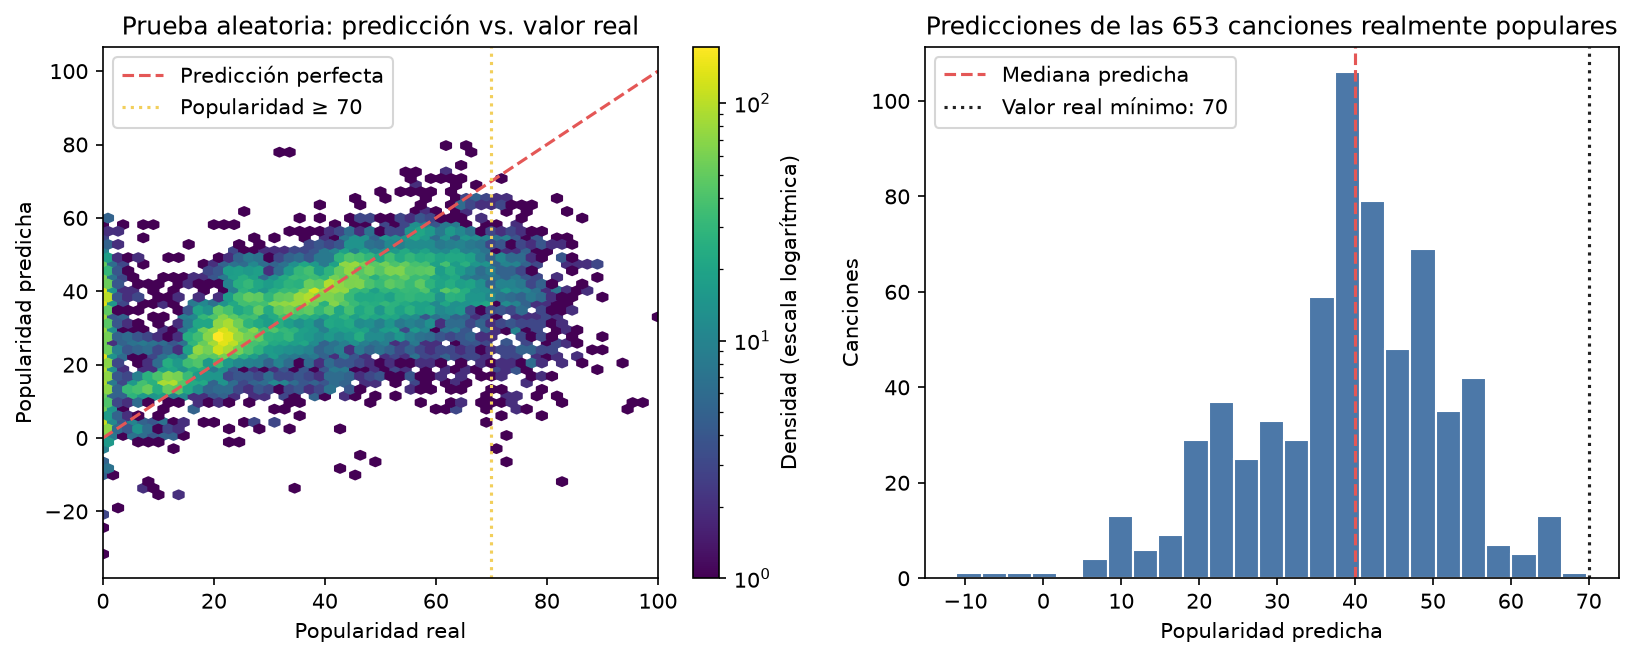
\includegraphics[width=\linewidth]{04a_lucas_predictions_vs_actual.png}
\caption{Valor predicho frente al real y distribución de predicciones de las 653 canciones realmente populares. La concentración intermedia explica subestimaciones grandes en el extremo alto.}
\label{fig:predictions}
\end{figure}

El modelo no contiene identidad de artista, fecha ni exposición promocional.
Esa ausencia es una explicación plausible de su dificultad para distinguir un
éxito excepcional o un cero entre canciones de géneros y perfiles parecidos,
pero los datos no permiten asignar una causa individual a cada error. El MAE
fue 14,198 en canciones \code{explicit=True} ($n=1.517$) y 11,704 en
\code{explicit=False} ($n=16.431$); los soportes son distintos y la diferencia
no demuestra un efecto de la explicitud.

El KPI utiliza una capacidad prefijada de 1.795 canciones (10\,\% redondeado
hacia arriba), popularidad real al menos 70 y desempate por \code{track_id}.
Precisión es la proporción de populares dentro de la lista; recall es la
proporción recuperada de las 653 populares de la prueba; lift divide la precisión
por la prevalencia de 3,64\,\% en \emph{esta muestra}.

\begin{table}[htbp]
\centering\small
\begin{tabular}{lrrrr}
\toprule
Ranking del 10\,\% & Populares halladas & Precisión & Recall & Lift \\
\midrule
Referencia mediana & 63 & 3,5\,\% & 9,6\,\% & 0,965 \\
Ridge completo & 159 & 8,9\,\% & 24,3\,\% & 2,435 \\
Ridge sin géneros & 136 & 7,6\,\% & 20,8\,\% & 2,082 \\
Árbol completo & 119 & 6,6\,\% & 18,2\,\% & 1,822 \\
Árbol sin géneros & 82 & 4,6\,\% & 12,6\,\% & 1,256 \\
\bottomrule
\end{tabular}
\caption{Ranking retrospectivo de las variantes declaradas. Porcentajes redondeados.}
\label{tab:kpi}
\end{table}

Al incluir géneros, Ridge recupera 23 populares adicionales respecto a la
variante sin géneros, y el árbol 37. El ranking de Ridge completo supera una
selección aleatoria de igual tamaño en esta muestra, pero deja fuera 494 de las
653 populares y selecciona 1.636 que no alcanzan el umbral. El lift no acredita
utilidad comercial: la fuente ya contiene popularidad histórica y el modelo
falla en los extremos absolutos.

\section{Perfiles no supervisados de canciones}

K-Means responde una pregunta distinta a la regresión: ¿aparecen perfiles
musicales reconocibles al agrupar canciones por sus atributos de audio? Se usaron
las 71.792 canciones del entrenamiento aleatorio, sin popularidad, géneros,
identificadores ni nombres en la matriz. Las diez variables numéricas declaradas
en la sección anterior se estandarizaron; los centroides se ajustaron en esa
escala. Para reducir la dependencia de una inicialización particular se fijó
semilla 42 y \code{n_init=10}. Se comparó $K=2,\ldots,8$ mediante inercia y
silueta estimada sobre 2.000 observaciones de entrenamiento.

\begin{figure}[htbp]
\centering
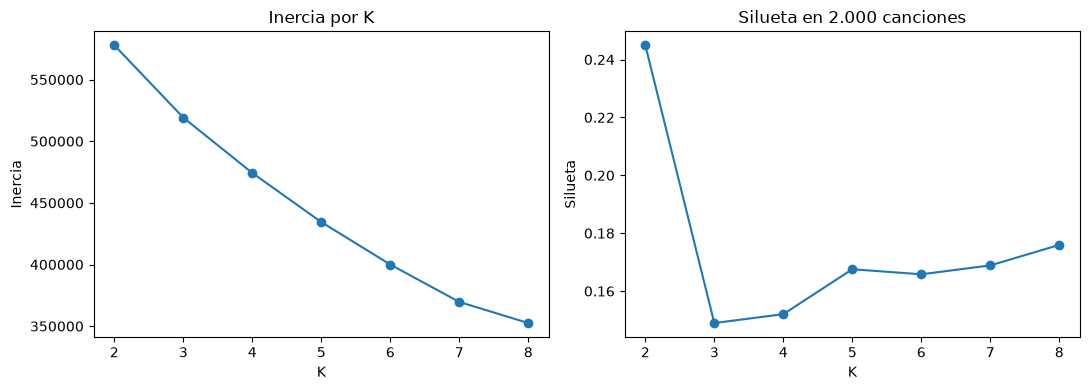
\includegraphics[width=0.87\linewidth]{04a_lucas_k_selection.png}
\caption{Inercia y silueta para $K=2,\ldots,8$. La curva apoya una solución descriptiva de dos grupos; la silueta máxima usada es 0,245. Figura extraída de la salida ejecutada del notebook 04a.}
\label{fig:k-selection}
\end{figure}

Se eligió $K=2$ por el balance entre lectura e indicador, con silueta 0,245.
Este valor indica separación limitada, no dos clases naturales de canciones.
Los perfiles se describieron con estadísticas en unidades originales y la
popularidad se consultó \emph{después} de agrupar, únicamente como descriptor.

\begin{table}[htbp]
\centering\small
\begin{tabular}{lrrrrrr}
\toprule
Grupo & Canciones & Energía & Acústica & Loudness & Bailabilidad & Popularidad mediana \\
\midrule
0 & 54.011 & 0,762 & 0,078 & $-6,140$ & 0,607 & 34 \\
1 & 17.781 & 0,295 & 0,828 & $-13,033$ & 0,468 & 29 \\
\bottomrule
\end{tabular}
\caption{Perfil del entrenamiento. Los valores acústicos son medianas descriptivas en escala original. La popularidad no intervino en K-Means.}
\label{tab:clusters}
\end{table}

El grupo 0 reúne principalmente canciones más enérgicas, menos acústicas y
con mayor \code{loudness}; el grupo 1, canciones más acústicas y suaves. La
mediana de popularidad difiere cinco puntos, sin que esta comparación pruebe que
pertenecer a un grupo cause mayor popularidad. PCA se utilizó solo para proyectar
la matriz estandarizada en dos ejes: ambos explican conjuntamente 44,1\,\% de
la varianza, por lo que la figura omite más de la mitad de la información.

\begin{figure}[htbp]
\centering
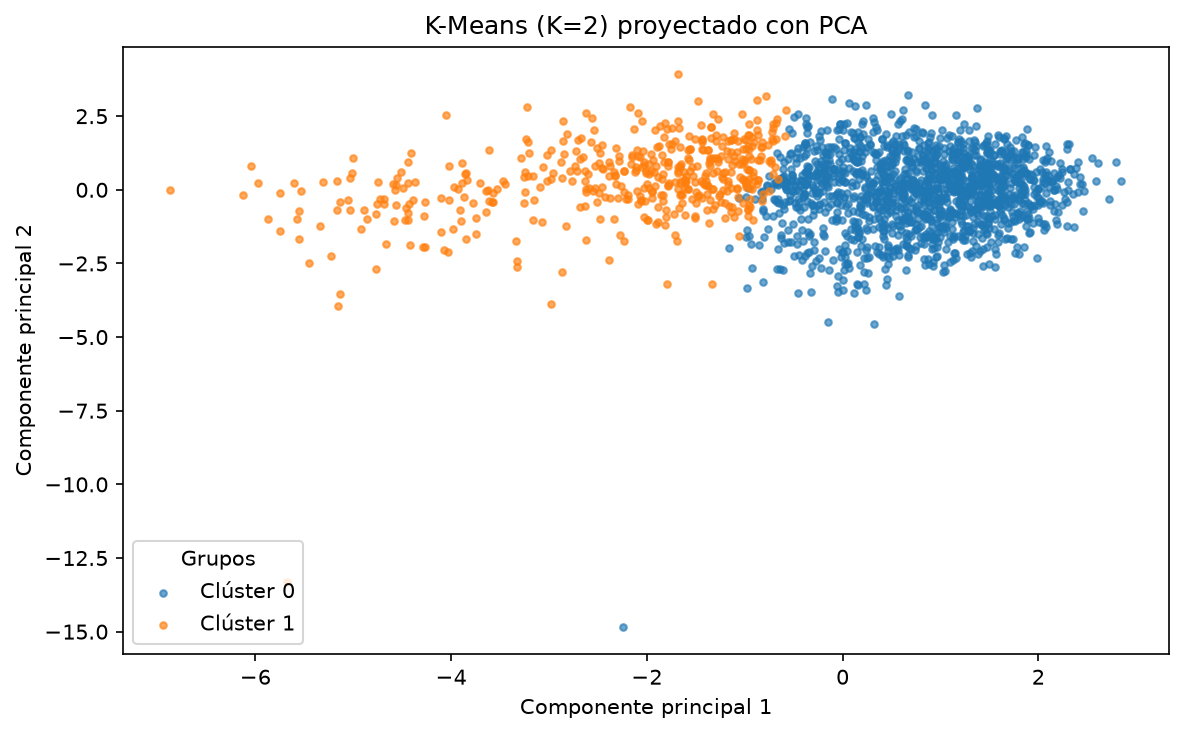
\includegraphics[width=0.82\linewidth]{04a_lucas_clusters_pca.png}
\caption{Proyección PCA de los dos grupos de K-Means. El solapamiento visible concuerda con la silueta moderada; la proyección no es evidencia de separación perfecta en diez dimensiones.}
\label{fig:clusters-pca}
\end{figure}

\subsection{Estabilidad de los perfiles}

Se repitió $K=2$ con el mismo entrenamiento y la misma semilla bajo dos cambios
aislados: transformar \code{duration_ms} con $\log(1+x)$ antes de escalar, y
retirar \code{loudness}. Los números de grupo son arbitrarios; la concordancia
se calculó después de alinear las etiquetas. ARI compara particiones sin
depender de esos nombres.

\begin{table}[htbp]
\centering\small
\begin{tabular}{lrrrr}
\toprule
Configuración & Silueta & ARI vs. base & Coincidencia & Tamaños \\
\midrule
Base, diez atributos & 0,245 & 1,000 & 100,000\,\% & 54.011 / 17.781 \\
Duración $\log(1+x)$ & 0,241 & 0,968 & 99,258\,\% & 53.954 / 17.838 \\
Sin \code{loudness} & 0,209 & 0,807 & 95,194\,\% & 51.769 / 20.023 \\
\bottomrule
\end{tabular}
\caption{Sensibilidad de la partición K-Means. ARI y coincidencia se comparan con la solución base sobre las mismas canciones.}
\label{tab:cluster-sensitivity}
\end{table}

Los dos perfiles siguen siendo reconocibles en ambas variantes. Retirar
\code{loudness} reduce la silueta y mueve más observaciones, señal de que esa
variable contribuye a la separación. Los resultados no validan estabilidad
frente a otras muestras, elecciones de $K$ o métodos de agrupamiento.

\section{Conclusiones y uso compartido}

Ridge completo es la mejor de las variantes supervisadas evaluadas para el
MAE de esta prueba aleatoria. La mejora depende marcadamente de géneros y
persiste, con límites, cuando se apartan artistas principales. La regresión
subestima sistemáticamente las canciones con popularidad al menos 70; por ello
el ranking sirve como filtro exploratorio retrospectivo, no como sustituto del
criterio humano. K-Means aporta un lenguaje descriptivo para explorar familias
acústicas, pero sus grupos no son categorías rígidas ni predicen por sí mismos
la popularidad.

Para el notebook integrador queda por medir si el ranking del 10\,\% cubre de
forma distinta los dos perfiles K-Means. \emph{Esta auditoría es una hipótesis,
no un resultado}.

\subsection{Traspaso a Ignacio y César}

Como trabajo posterior, una evaluación temporal requeriría fechas válidas;
extrapolar a Spotify exige una muestra con frecuencias naturales de géneros.

\begin{enumerate}
\item Reproducir el notebook 04a siguiendo \path{docs/ea2/lucas.md}; verificar
la huella de la fuente, los 89.740 \code{track_id} únicos y la huella de la
prueba común antes de comparar resultados.
\item Reutilizar las funciones del protocolo compartido y reservar la misma
prueba aleatoria. Seleccionar hiperparámetros en validación propia; el
diagnóstico agrupado exige una selección nueva dentro de esa partición.
\item Llevar al notebook 05 los resultados de las Tablas~\ref{tab:random-test},
\ref{tab:artist-test}, \ref{tab:kpi} y \ref{tab:cluster-sensitivity}, con sus
soportes y límites. Contrastar allí los enfoques de los tres integrantes antes
de redactar una conclusión de equipo.
\item En la revisión cruzada, explicar por qué la señal de género puede estar
amplificada por el muestreo, qué significa que todos los populares de prueba
reciban predicción inferior a 70, cómo se calculó el lift y por qué la silueta
0,245 obliga a una interpretación prudente de los grupos.
\end{enumerate}

Las figuras de modelamiento y clustering proceden del notebook 04a; las dos
figuras de contexto proceden del EDA de EP1. El archivo principal de este
informe es \path{docs/ea2/informe_lucas/main.tex} y el PDF compilado queda en
esa misma carpeta. El código, notebook, imágenes y documento son archivos
locales de la rama \code{feature/ea2-modeling-lucas} hasta que el equipo los
integre. Así, la revisión puede hacerse sobre evidencia trazable sin confundir
el informe individual con la entrega conjunta.

\end{document}
